\chapter{Erweiterte Flugtests: Avoidance}
Für die Flugtests mit realer Hardware kommt wieder ein \gls{rpi} Model 3B+ zum Einsatz. Innerhalb dieses Kapitels wird dessen Software mit komplett neuem Betriebssystem eingerichtet. Anschließend werden die Ultraschallsensoren überprüft. Danach nochmals kleine Anpassungen zu \textit{Avoidance} vorgenommen und ein Feldversuch durchgeführt. Da keine Berechtigung zum Fliegen der Drohne vorliegt kann dies nur als Übung angesehen werden.

\section{Einrichtung des Raspberry Pi Model 3 B+}
Der \gls{rpi} ist wie in [Referenz Bild Anfang] gezeigt auf die Drohne montiert. Peripherieverbindungen mit dem Flugcontroller (via \acrshort{uart}) und dem Arduino (via \acrshort{i2c}) sind vorhanden.\newline
Als Betriebssystem wurde Raspberry Pi OS Lite (64 bit)\footnote{\url{https://www.raspberrypi.com/software/operating-systems/\#raspberry-pi-os-64-bit}} installiert. Dieses verwendet keine graphische Oberfläche (Desktop) sondern nur Kommandozeile. Damit ist es kleiner in Speicher- und Ressourcenbedarf. Es ist notwendig die 64-Bit Version zu verwenden, denn nur diese wird von \acrshort{ros} auf der Architektur \enquote{arm} unterstützt.\newline
Beim Schreiben des Betriebssystems wird bereits die Funktionalität \enquote{ssh} aktiviert, um später Fernzugriff zu erlauben. Benutzername und Passwort werden gewählt wie im ersten Projektteil: Benutzername \enquote{pi} und Passwort \enquote{dhbw1234}. Zur Einrichtung wird der \gls{rpi} per Netzwerkkabel angeschlossen und eine Konsole mittels \textit{ssh} geöffnet.\newline
Um weitere Schritte der Einrichtung nachvollziehbar zu gestalten, wurden diese als Script zusammengefasst. Dieses ist im Anhang unter \ref{listing:setup_rpi.sh} abgedruckt. Die Schritte zusammengefasset sind:
\begin{itemize}
    \item Installieren von Drittprogrammen um die Bedienung zu Erleichtern
    \item Einrichten \gls{wlan}-Hotspot wie in \cite[Kapitel 6.12]{wirthErweiterungBestehendenDrohne2022a}\footnote{bzw. \url{https://www.elektronik-kompendium.de/sites/raspberry-pi/2002171.htm}}
    \item Installieren von Docker
    \item Vergrößern der Swap-Datei
\end{itemize}

Die Swap-Datei steht als Erweiterung des Arbeitsspeichers als Speicher auf der Speicherkarte zur Verfügung. Die $512MB$ Arbeitsspeicher des \gls{rpi} reichen an vielen Stellen nicht aus. Ohne diese Anpassung kommt es bei der Verwendung von Docker oder bei Kompilierung von C-Projekten (im Docker Container wird später das \textit{Avoidance}-Modul kompiliert) zu Fehlern aufgrund unzureichenden Speichers.\newline
Weiterhin werden manuelle Anpassungen innerhalb des Programmes \enquote{raspi-config} vorgenommen:
\begin{itemize}
    \item Aktivieren \acrshort{uart}-Interface, deaktivieren \enquote{Debug-Konsole} (im selben Schritt wie \gls{uart})
    \item Aktivieren \acrshort{i2c}-Interface
    \item Erweitern des Dateisystems
\end{itemize}

\section{Starten des Docker Containers}
Nach Einrichtung der Software wird ein entsprechender Container mit der Software \acrshort{ros}, \textit{Avoidance} und Einspeisung der Ultraschall-Sensordaten gebaut. Die entsprechende \textit{Dockerfile} befindet sich auf der Speicherkarte des \gls{rpi}. Die notwendigen Schritte auf der Kommandozeile sind wie folgt:
\begin{minted}{bash}
    # Image bauen
    docker build -t im_ros_drohne .
    # Container mit Hardwarezugriff starten
    docker run -it --privileged --net host ros_drohne
    # Oder Container erst bauen, dann starten
    docker container create --privileged --net host --name ros_test ros_drohne
    docker start ros_test # Startet 'roscore' im Container

    # Auf dem Container, am besten innerhalb einer Screen-Session:
    # Bekanntmachen eigene IP als ROS-Master
    export ROS_MASTER_URI=http://192.168.4.1:11311/
    # Bekanntmachen eigene IP
    export ROS_IP=192.168.4.1
    # Abhaengigkeiten fuer ROS-Packete initialisieren
    source ros_entrypoint.sh
    # Abhaengigkeiten fuer Benutzer-Packete initialisieren
    source catkin_ws/devel/setup.sh
    
    # Finale Schritte zum Starten der Teilprogramme
    # Mavros stellt UART Verbindung zur Drohne her
    # und Server fuer Verbindung mit PC bereit
    roslaunch mavros px4.launch fcu_url:=/dev/serial0:921600 gcs_url:=tcp-l://
    # Sensordaten auslesen und Topic publizieren
    rosrun ultrasensor sensor_interface.py
    # Local-Planner starten
    # roslaunch local_planner local_planner_hw.launch
\end{minted}

Der Ablauf einen zuvor gebauten Container zu starteten ist in Bild \ref{fig:avoid_container_start} gezeigt. Soll ein weiteres Programm im Container ausgeführt werden, kann dies mit \texttt{docker exec}, wie in Bild \ref{fig:avoid_container_exec} dargestellt, durchgeführt werden.

\begin{figure}[!ht]
    \centering
    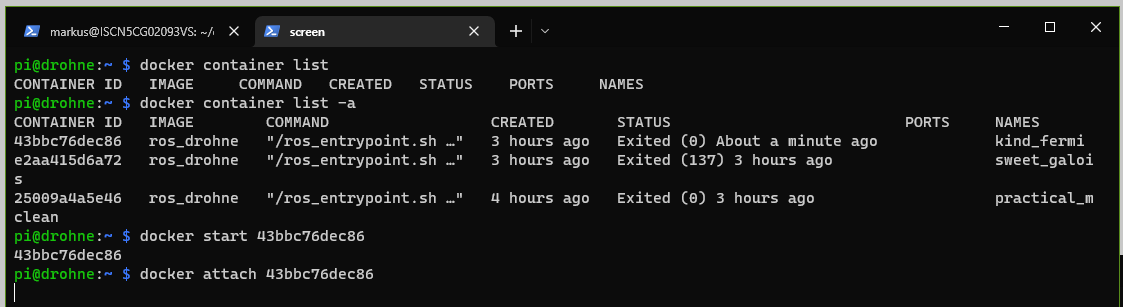
\includegraphics[width=0.6\linewidth]{images/avoid_container_start.png}
    \caption[Starten vorhandener Docker-Container]{Starten vorhandener Docker-Container: Mittels \texttt{docker ps -a} werden alle vorhandenen Container angezeigt. Anschließend kann ein Container gestartet werden. Ohne weitere Argumente beendet sich dieser relativ schnell, weil kein Programm gestartet wurde. Mit \texttt{docker attach} wird ein Benutzer eingewählt und dieses Verhalten unterdrückt}
    \label{fig:avoid_container_start}
\end{figure}
\begin{figure}[!ht]
    \centering
    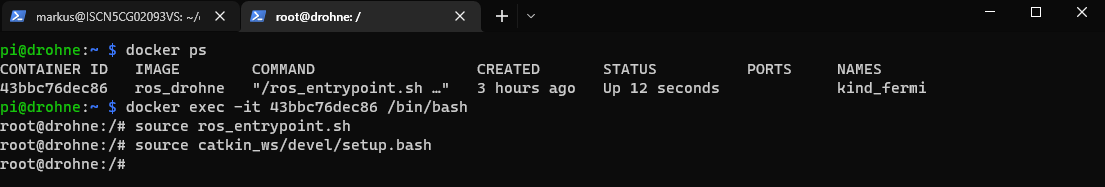
\includegraphics[width=0.6\linewidth]{images/avoid_container_exec.png}
    \caption[Ausführen von Programmen auf Docker-Container]{Ausführen von Programmen auf Docker-Container: Mittels \texttt{docker ps} können laufende Container angezeigt werden. Anschließend kann ein Programm (hier die Konsole) auf dem Container gestartet werden. Es ist für jede neue Instanz notwendig die Initialisierungsdateien auszuführen}
    \label{fig:avoid_container_exec}
\end{figure}

\section{Überprüfen der Ultraschallsensoren}
Nachdem der Container gestartet ist, kann sich ein zweiter PC mit dem \gls{wlan}-Hotspot verbinden. Auf diesem steht eine komplette \acrshort{ros}-Noetic Umgebung mitsamt graphischen Programmen bereit. Um mit dem \gls{rpi} in Verbindung zu treten, müssen 2 Umgebungsvariablen korrekt gesetzt werden:
\begin{minted}{bash}
    # Bekanntmachen IP des RPI als ROS-Master
    export ROS_MASTER_URI=http://192.168.4.1:11311/
    # Bekanntmachen eigene IP
    export ROS_IP=192.168.4.3
\end{minted}

Anschließend können Programme wie \enquote{rqt} oder \enquote{rviz}\cite[Kapitel 5.2ff]{markusreinErweiterungBestehenderDrohnen2023} gestartet werden.\newline
Zum visualisieren wird die in \textit{Avoidance} enthaltene Konfigurationsdatei für \textit{rviz} importiert. Zusätzlich werden die Punkte der Ultraschallsensoren sensoren hinzugefüft. Das Ergebnis ist in Bild \ref{fig:avoid_plan_sensors} zu sehen.

\begin{figure}[!ht]
    \centering
    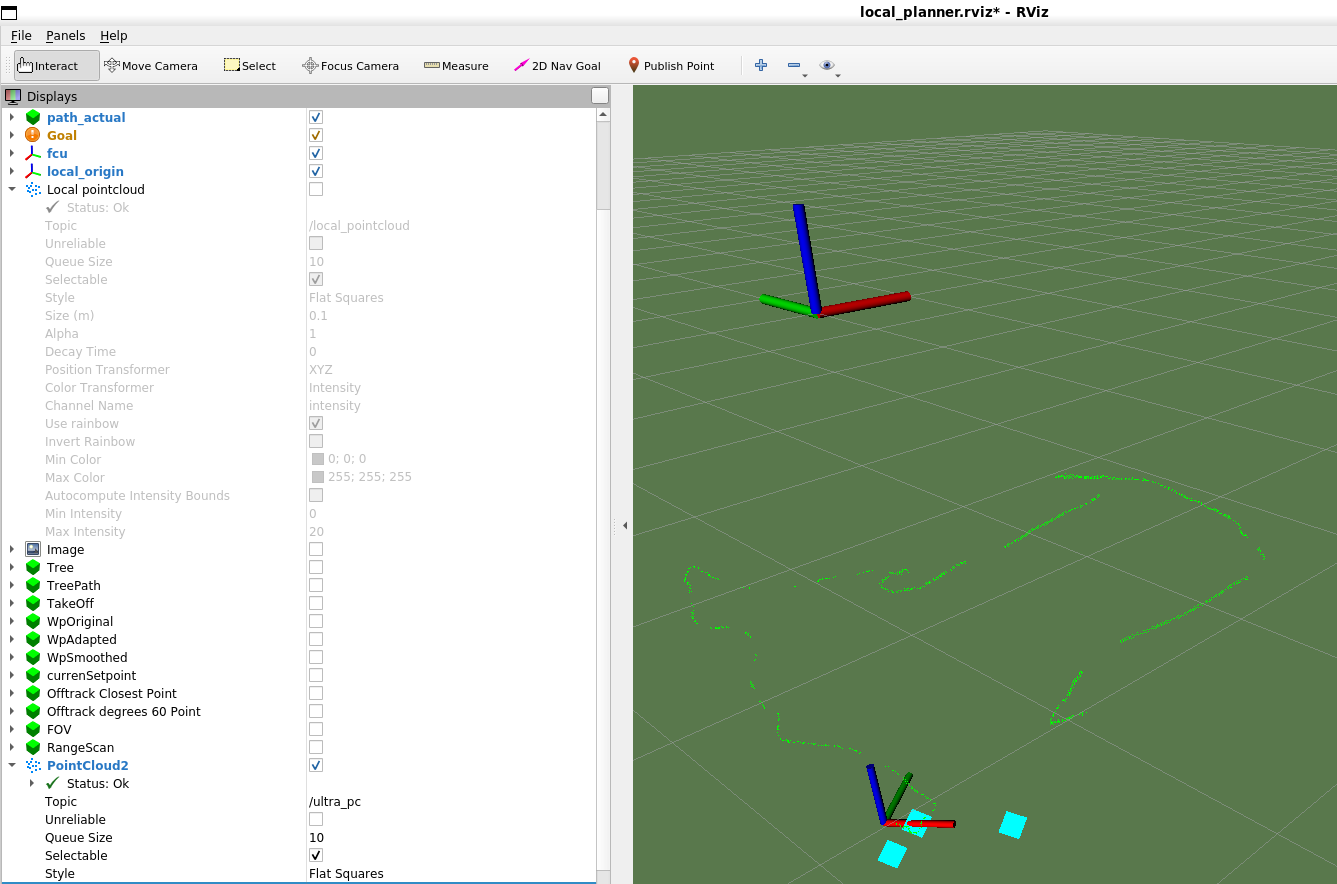
\includegraphics[width=0.7\linewidth]{images/avoid_plan_sensors.png}
    \caption[rviz mit Drohne und Punktwolke]{rviz mit Drohne und Punktwolke: im unteren Bildbereich das Koordinatensystem der Drohne. Dieses wurde bereits vom Ursprung wegbewegt. 2 blaue Punkte als Sensordaten vor der Drohne (in Richtung roter Achse), 1 blauer Punkt Sensordaten unter der Drohne. Kein blauer Punkt über der Drohne denn Abstand zur Decke ist größer als $4m$ (Test durchgeführt unter freiem Himmel)}
    \label{fig:avoid_plan_sensors}
\end{figure}

\section{Überprüfen Funktionalität Avoidance}
Um \textit{Avoidance} als Gesamtsystem zu starten, wurde im Container die Datei \enquote{local\_planner\_hw.launch} angelegt. Sie ist hinterlegt in Listing \ref{listing:local_planner_hw.launch} und enthält gleichzeititg die Konfiguration für \textit{mavros} und die Sensorverarbeitung der Ultraschallsensoren. Ein weiteres Script wurde geschrieben um die Startdatei auszuführen und somit alle notwendigen Prozesse zu automatisieren. Hinterlegt in \ref{listing:setup_container.sh}, ist es auszuführen per \texttt{source setup\_container.sh}, wodurch sich alles notwendige startet.\newline

Eine beispielhafte Ausgangssituation ist gezeigt in Bild \ref{fig:avoid_local_plan_pathing}. Die Drohne steht ohne erkennbare Hindernisse nahezu im Ursprung und wartet auf Anweisungen. Erhält sie das Kommando zum abheben (entweder per QGroundControl oder Kommandozeile \texttt{rosrun mavros mavsys mode -c OFFBOARD \&\& rosrun mavros mavsafety arm}) fliegt sie auf den gelben Zielpunkt zu.

\begin{figure}[!ht]
    \centering
    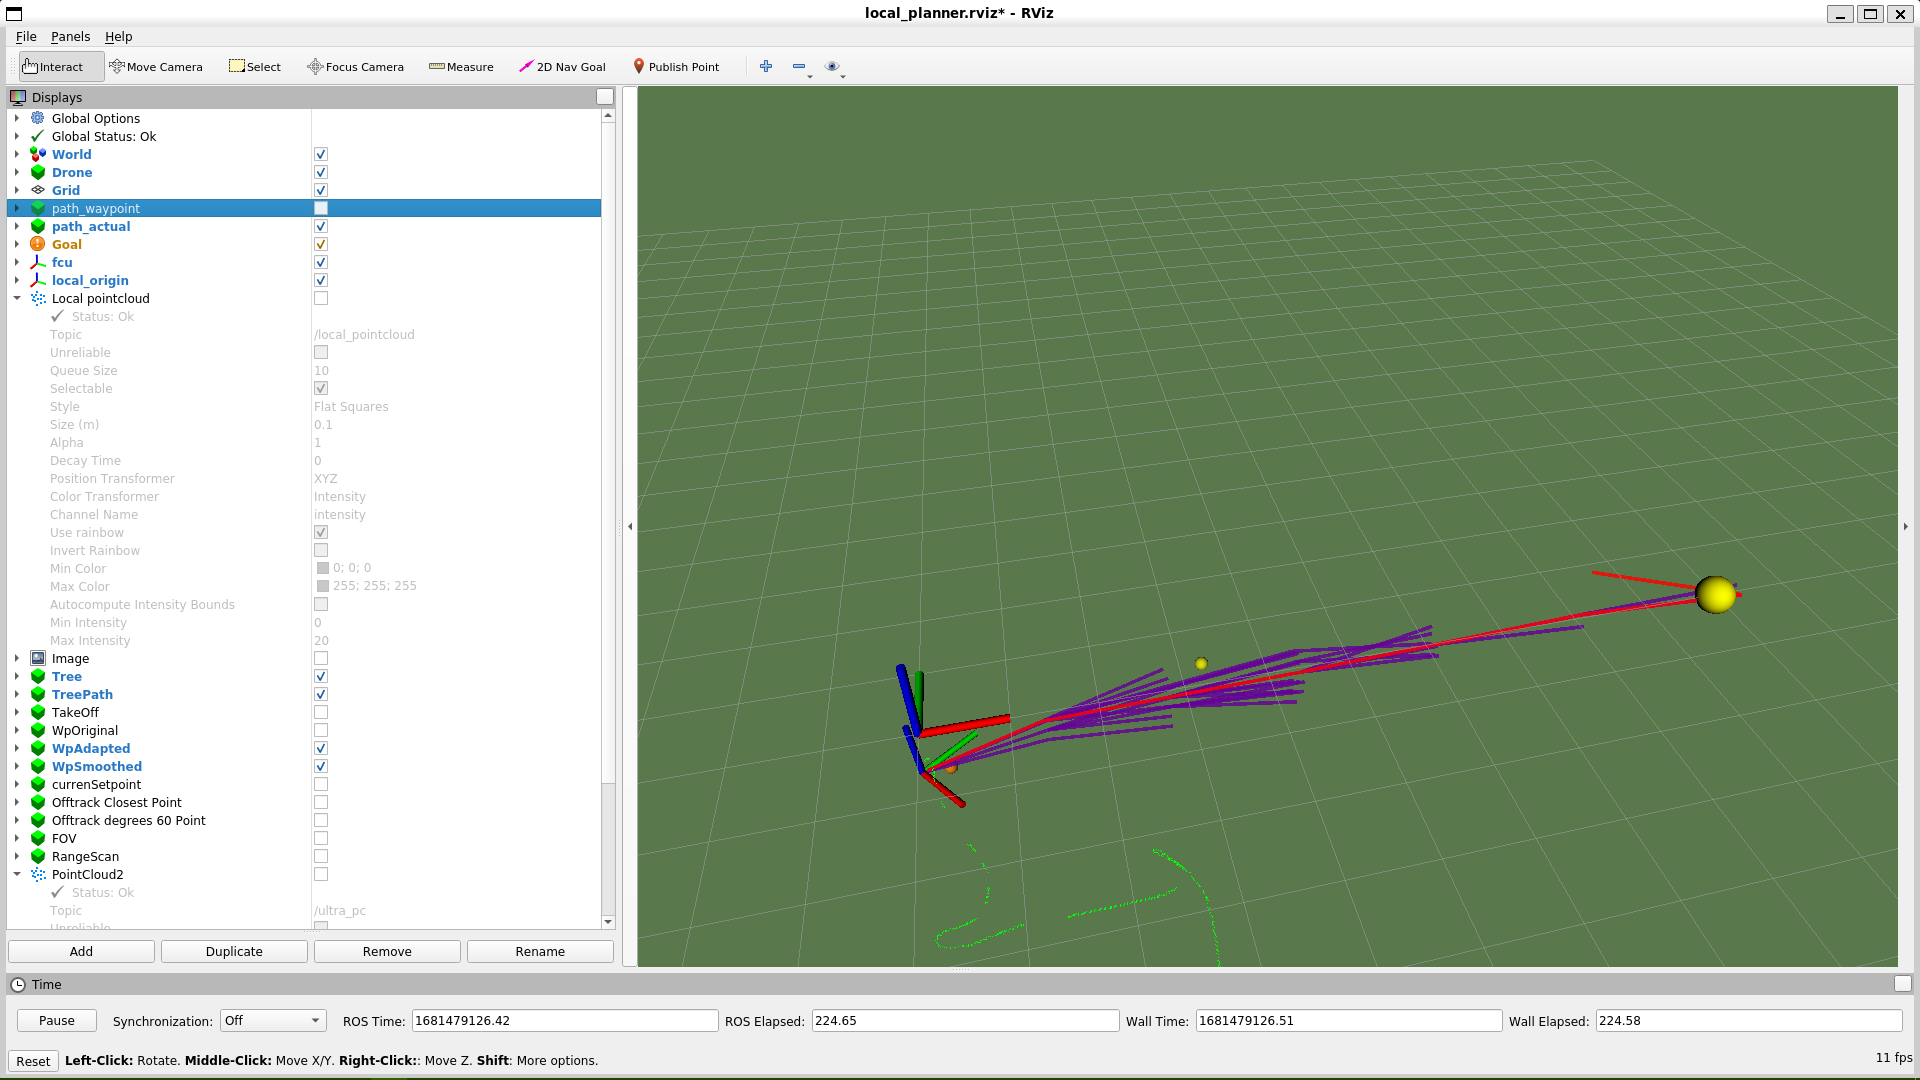
\includegraphics[width=0.7\linewidth]{images/avoid_local_plan_pathing.png}
    \caption[rviz mit gestartetem Local-Planner]{rviz mit gestartetem Local-Planner: von der derzeitigen Position (unteres Koordinatensystem) wird ein Weg zum gelben Zielpunkt entlang der roten Linie geplant. Die lilanen Abschnitte sind potenzielle abzufliegende Wegstücke}
    \label{fig:avoid_local_plan_pathing}
\end{figure}

Werden von den Sensoren Hindernisse erkannt, so werden vom Local-Planner neue Wegvorgaben ausgegeben, meist dreht die Drohne und versucht an diesen vorbei zu fliegen. Das Verhalten ist gezeigt in Bild \ref{fig:avoid_local_plan_correct}.

\begin{figure}[!ht]
    \centering
    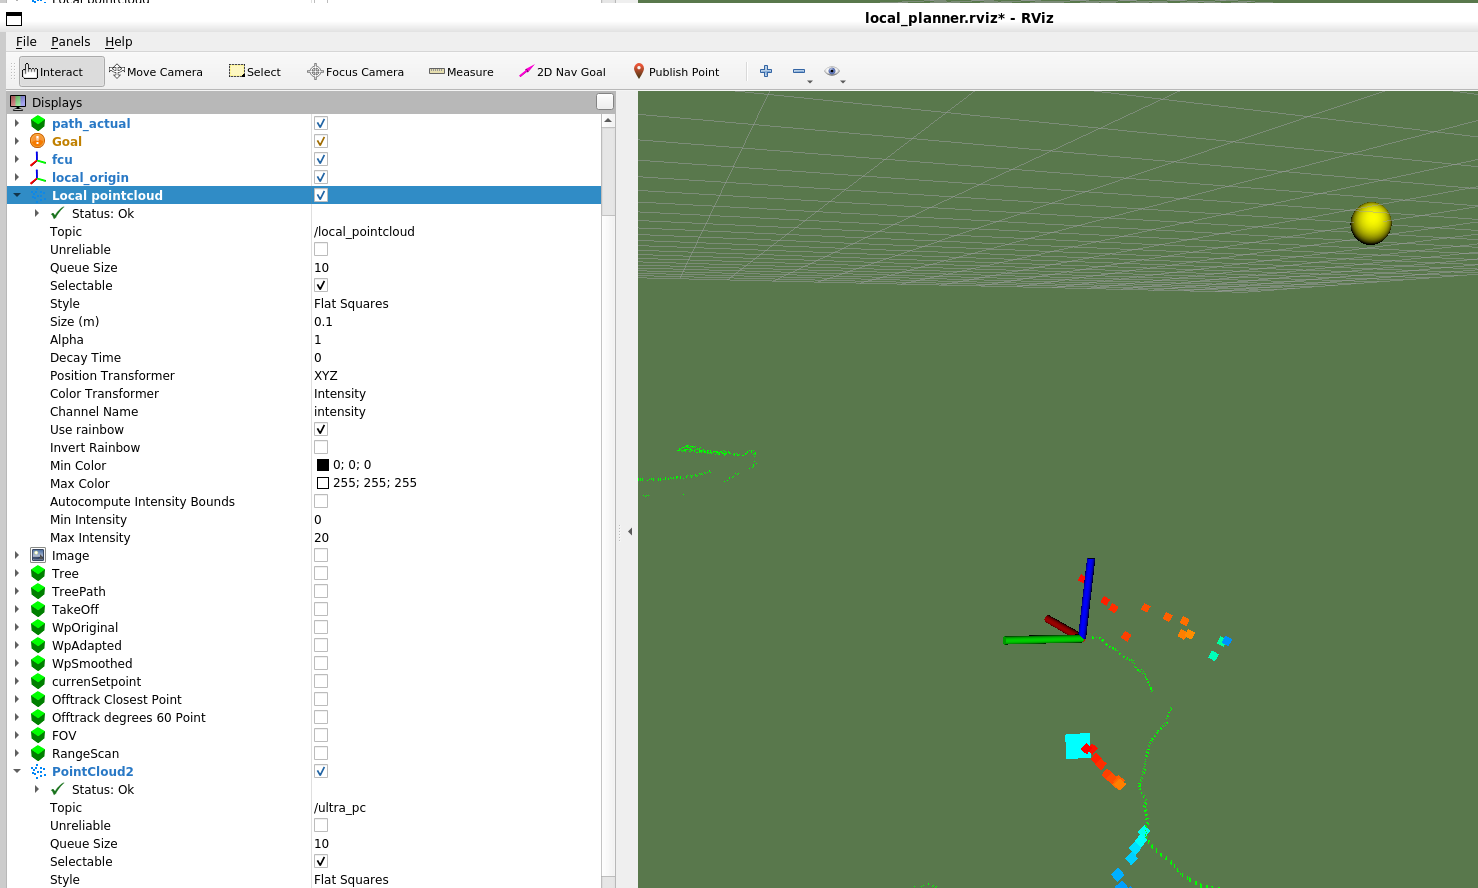
\includegraphics[width=0.7\linewidth]{images/avoid_local_plan_correct.png}
    \caption[rviz mit gestartetem Local-Planner 2]{rviz mit gestartetem Local-Planner 2: kleine Punkte verdeutlichen die Historie erkannter Hindernisse. Bläulich gefärbt sind die ältesten, rötlich gefärbt die neusten Punkte. Da die Drohne über dem Boden gehalten wurde, wird unter ihr ein Pfad, mit dem großen hellblauen Punkt als aktueller Messwert des Sensors, erkannt. Rechts der Drohne waren auch Hindernisse, aber sie wurde von oben gesehen gegen den Uhrzeigersinn gedreht}
    \label{fig:avoid_local_plan_correct}
\end{figure}
